\begin{enumerate}
	\item L'administrateur se connecte au site avec ses identifiant. 
	\item Un nouveau bouton de navigation apparait dans la bar de navigation. 
	\item L'administrateur clique sur le bouton \textit{Admin}
	\item Il sélectionne \textit{Type Session} dans le menu déroulant. 
	\item L'administrateur atterris sur la page de gestion des type de sessions. 
	\item Il clique sur \textit{Ajout d'une session +}
	\item Un formulaire apparait et il le remplis avec les bonne information (jour - heure [hh:mm])
	\item Il clique sur \textit{ok} 
\end{enumerate}

\vspace{\baselineskip}
\begin{figure}[h]
	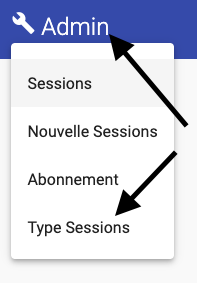
\includegraphics[width=0.3\textwidth,center]{Figures/us12-1}
	\caption{Bouton de navigation de l'administrateur}
\end{figure}

\newpage
\begin{figure}[h]
	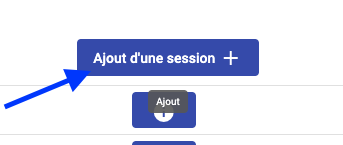
\includegraphics[width=0.5\textwidth,center]{Figures/us12-2}
	\caption{Bouton d'ajout d'un type de session}
\end{figure}

\vspace{\baselineskip}
\begin{figure}[h]
	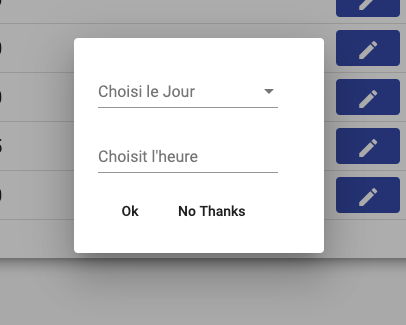
\includegraphics[width=0.5\textwidth,center]{Figures/us12-3}
	\caption{Page d'ajout du type de session}
\end{figure}

\vspace{\baselineskip}
\subsubsection{Gestion des erreurs}
	\begin{itemize}
		\item 2 types de session identique ne peuvent exister, l'ors de la creation d'un type de session une vérification se fait et si le type de session existe deja une erreur apparait.
		\item Si une erreur apparait durant la création du type des sessions, elle s'affichera au dessus du formulaire. 
	\end{itemize}

\newpage
\subsubsection{Diagramme de séquence}
	\begin{figure}[h]
		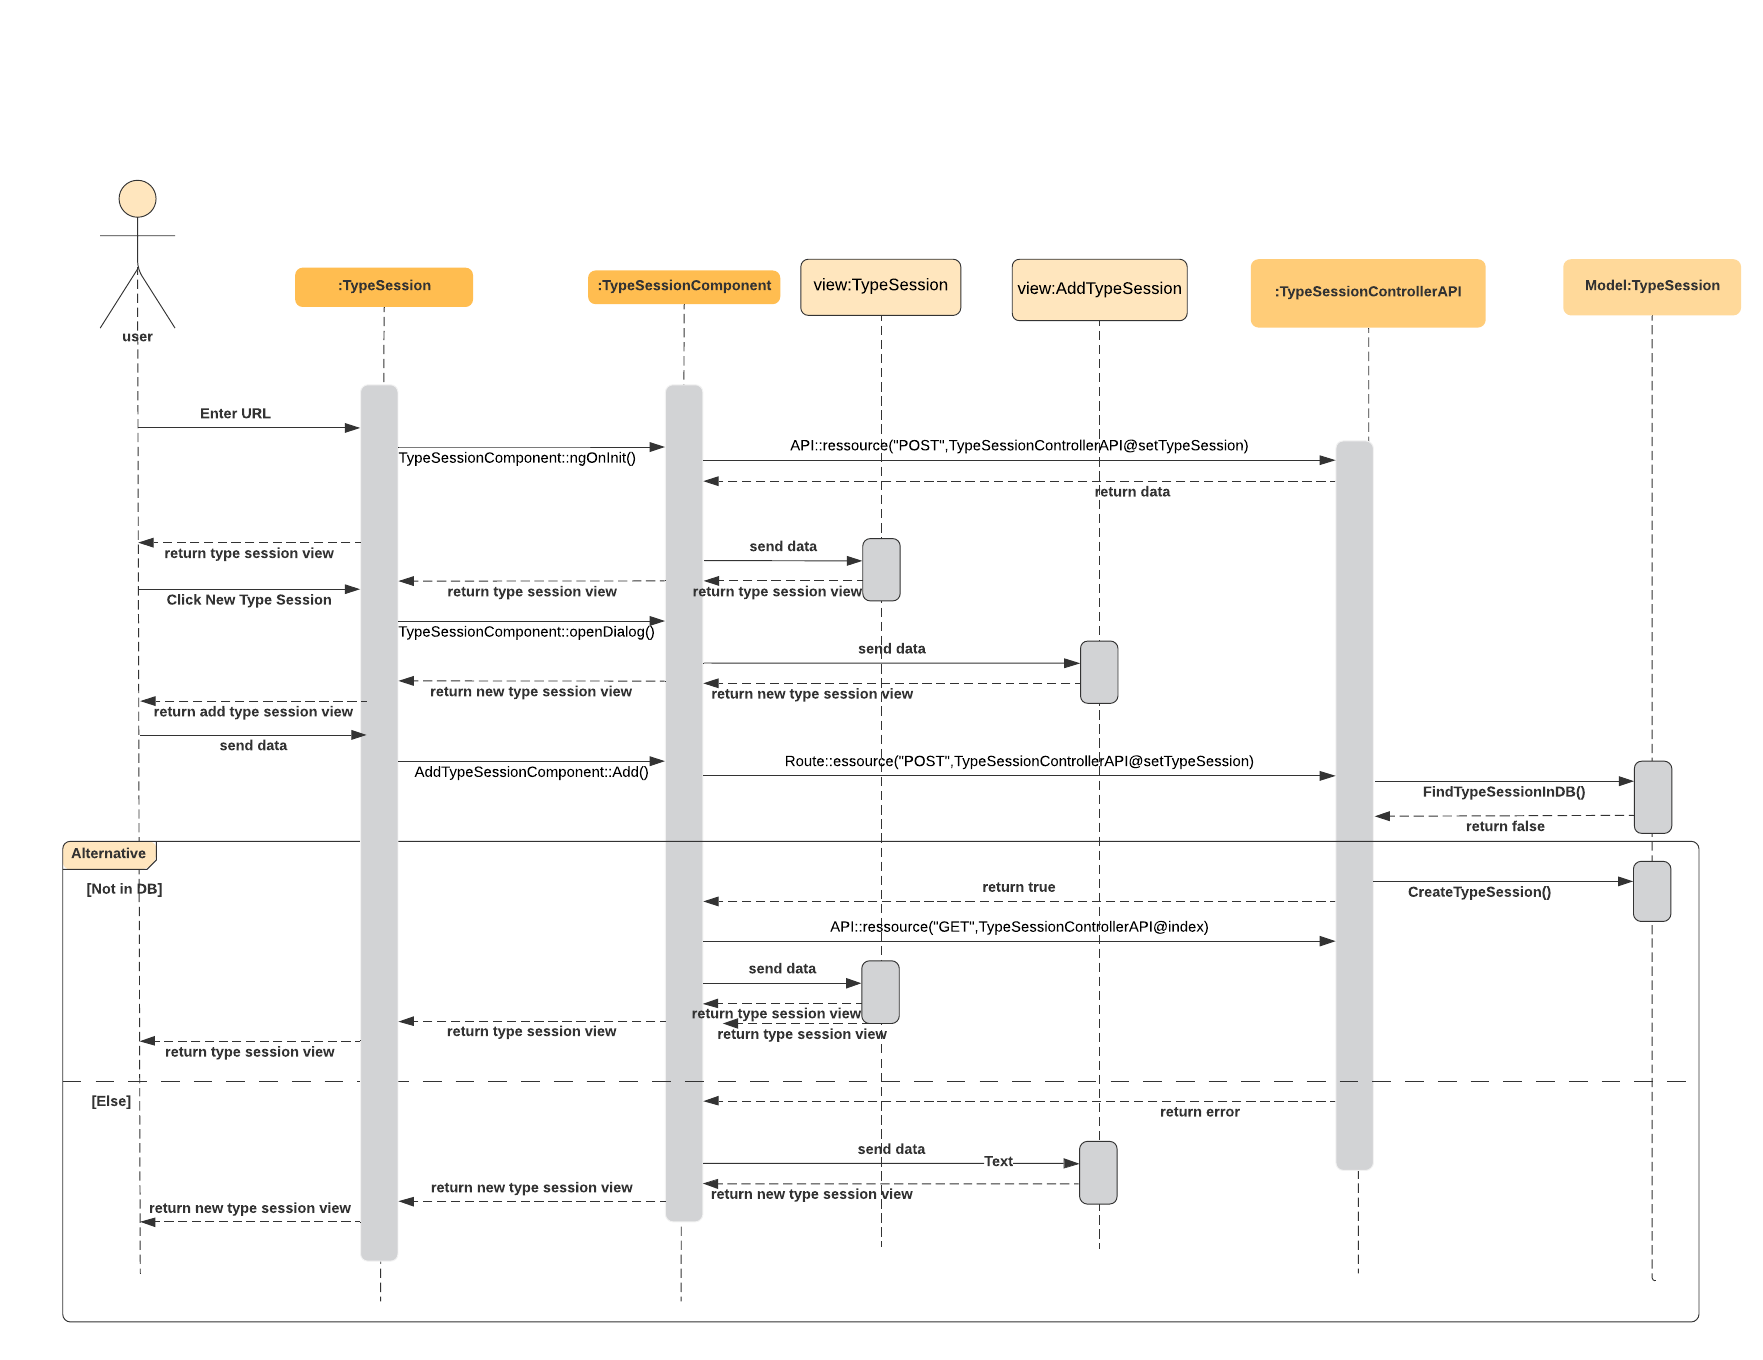
\includegraphics[width=0.9\textwidth,center]{Diagramme/sequence-us12}
		\caption{Diagramme de séquence de l'ajout d'un type de session}
	\end{figure}

\subsubsection{Script concerné}
	\begin{itemize}
		\item \href{https://github.com/victorsmits/Aquabike/blob/master/backend/src/Controller/API/RegistrationControllerApi.php}{RegistrationControllerApi.php}
		\item \href{https://github.com/victorsmits/Aquabike/blob/master/backend/src/Entity/TypeSession.php}{TypeSession.php}
		\item \href{https://github.com/victorsmits/Aquabike/blob/master/frontend/src/app/type-session/add-type-session.component.ts}{add-type-session.component.ts}
		\item \href{https://github.com/victorsmits/Aquabike/blob/master/frontend/src/app/type-session/add-type-session.component.html}{add-type-session.component.html}
	\end{itemize}
